\section{Experimental Setup and Results}
\label{sec:experiments}

\subsection{Dataset 1: Snowy Scenes}
\label{sec:dataset-snowy}

We evaluate on Snowy Scenes~\cite{SnowyScenes2026}, a multimodal driving dataset captured entirely in real winter conditions and distributed as a single $\sim$49\,GB archive, read lazily rather than extracted to disk given its $\sim$93\,GB uncompressed footprint. It contains 5{,}027 frames across three splits (3{,}016 train / 1{,}005 val / 1{,}006 test), with per-frame RGB camera images, 128-beam LiDAR point clouds, 3D object boxes, and per-point semantic segmentation labels across 29 classes (not consumed here, since the detector's head has no segmentation output).

Snowy Scenes' three weather categories -- \texttt{accumulated}, \texttt{highway}, and \texttt{falling} -- are all already-snowy driving, so no dry/clear split exists to serve as a calibration baseline or as the nominal side of an onset transition. Severity also does not ramp monotonically within a category: sampling the ground-truth per-point ``snow'' semantic class fraction across a timestamp-ordered \texttt{falling} sequence shows real but noisy fluctuation ($0.002$--$0.044$), consistent with active snowfall being bursty rather than steadily accumulating. What the data does support is a real, physically grounded severity contrast \emph{across} categories: the mean per-point ``snow''-class fraction per category gives $\texttt{accumulated} = 0.0001 < \texttt{highway} = 0.0041 < \texttt{falling} = 0.0119$, an ordering with a clear physical explanation -- \texttt{falling} captures active, airborne snowfall, which LiDAR registers as spurious near-range returns, while \texttt{accumulated} is settled snow on surfaces rather than particles in the air. We use this cross-category contrast, rather than a within-sequence transition, as the basis for the onset construction: a nominal (held-out \texttt{accumulated}) prefix spliced with a degraded (\texttt{falling}) suffix at a known onset index. Every individual frame on both sides of the transition is real sensor data; only the splice point itself is a construction, since Snowy Scenes' own sequences do not contain a within-sequence weather transition -- an assembled proxy for a naturally occurring onset, and we flag that openly as a limitation of the evaluation protocol.

We train the detector for 5 epochs on the real train split under its Adversarial Consistency Training objective, on a single local NVIDIA RTX 5000 Ada GPU, at $128\times128$ BEV resolution, batch size 4, Adam with learning rate $10^{-4}$; training loss converges from $\approx 2.3$ to $\approx 0.008$.

\subsubsection{A Real Negative Result: the CCP Covariate}
\label{sec:ccp-negative}

Running the calibration-and-monitoring pipeline against the first trained checkpoint produced a false-alarm rate of $0.0$ across every tested $\delta$ and detection delays that were numerically identical between the covariate-informed and covariate-blind bettors, to every digit the operating curve reports. Sampling the CCP consistency score $S$ directly across a real onset stream with the trained model showed why: $S$ had collapsed to $\approx 0.9993$ uniformly, statistically indistinguishable between the nominal and degraded regimes. Tracing the cause led to the training code rather than to anything in the monitoring code itself: the CCP contrastive loss was being computed once per training step, on the clean forward pass, against an all-ones mask -- real, synchronized frames have no annotated camera$\leftrightarrow$LiDAR mismatch to supervise against -- and the two additional CCP forward passes the training loop already computes, on adversarially perturbed features, were never fed into that loss with a mismatched target. Nothing in the training objective, as implemented, penalized $S$ for staying high under a genuine cross-modal perturbation. We fixed this by also supervising the two adversarial branches with the same CCP loss against a mismatched target, since a perturbed feature pair is a real cross-modal mismatch by construction, and retrained from scratch.

After the fix, $S$ varies again -- but in the wrong direction for this task. Figure~\ref{fig:qualitative-multi} shows this directly on six real frames rather than a single pair: three \texttt{accumulated} (nominal) and three \texttt{falling} (degraded) val-split frames, spread across each category's frame pool rather than consecutive samples, with camera image, LiDAR BEV occupancy, and the CCP disagreement heatmap for each. The per-frame mean disagreement is $0.611$, $0.583$, $0.576$ for the three \texttt{accumulated} frames and $0.564$, $0.559$, $0.573$ for the three \texttt{falling} frames -- category means of $0.590$ (nominal) versus $0.565$ (degraded), consistently the opposite of the ordering the covariate is meant to provide, and consistent enough across six independent frames that this is not an artifact of the single frame pair used in a smaller-scale version of this evaluation. Table~\ref{tab:snowy-results} reports the full operating curve this produces: the covariate-blind backbone detects the true weather onset within 3 to 10 frames depending on the false-alarm budget, with zero false alarms at every budget tested, while the covariate-informed bettor -- with disagreement now uniformly high across both regimes rather than rising specifically at onset -- bets aggressively throughout the stream and never accumulates enough evidence to alarm within the evaluation window, at any of the three $\delta$ tested. Our best explanation is that the fix supervises $S$ using adversarially perturbed features as the mismatch target, appropriate for the detector's own adversarial-robustness objective, but an $\ell_\infty$-bounded adversarial perturbation is a qualitatively different feature-space disturbance than real snowfall produces, and teaching $S$ to recognize the former does not obviously transfer to the latter. This generalizes beyond one architecture: a signal trained under an invariance objective is, by construction, in tension with reusing it as a leading indicator of degradation, which needs exactly the sensitivity the training objective suppressed -- a caution worth stating plainly for any future work that considers repurposing an internal robustness or consistency signal as an external monitoring covariate.

\begin{figure}[t]
\centering
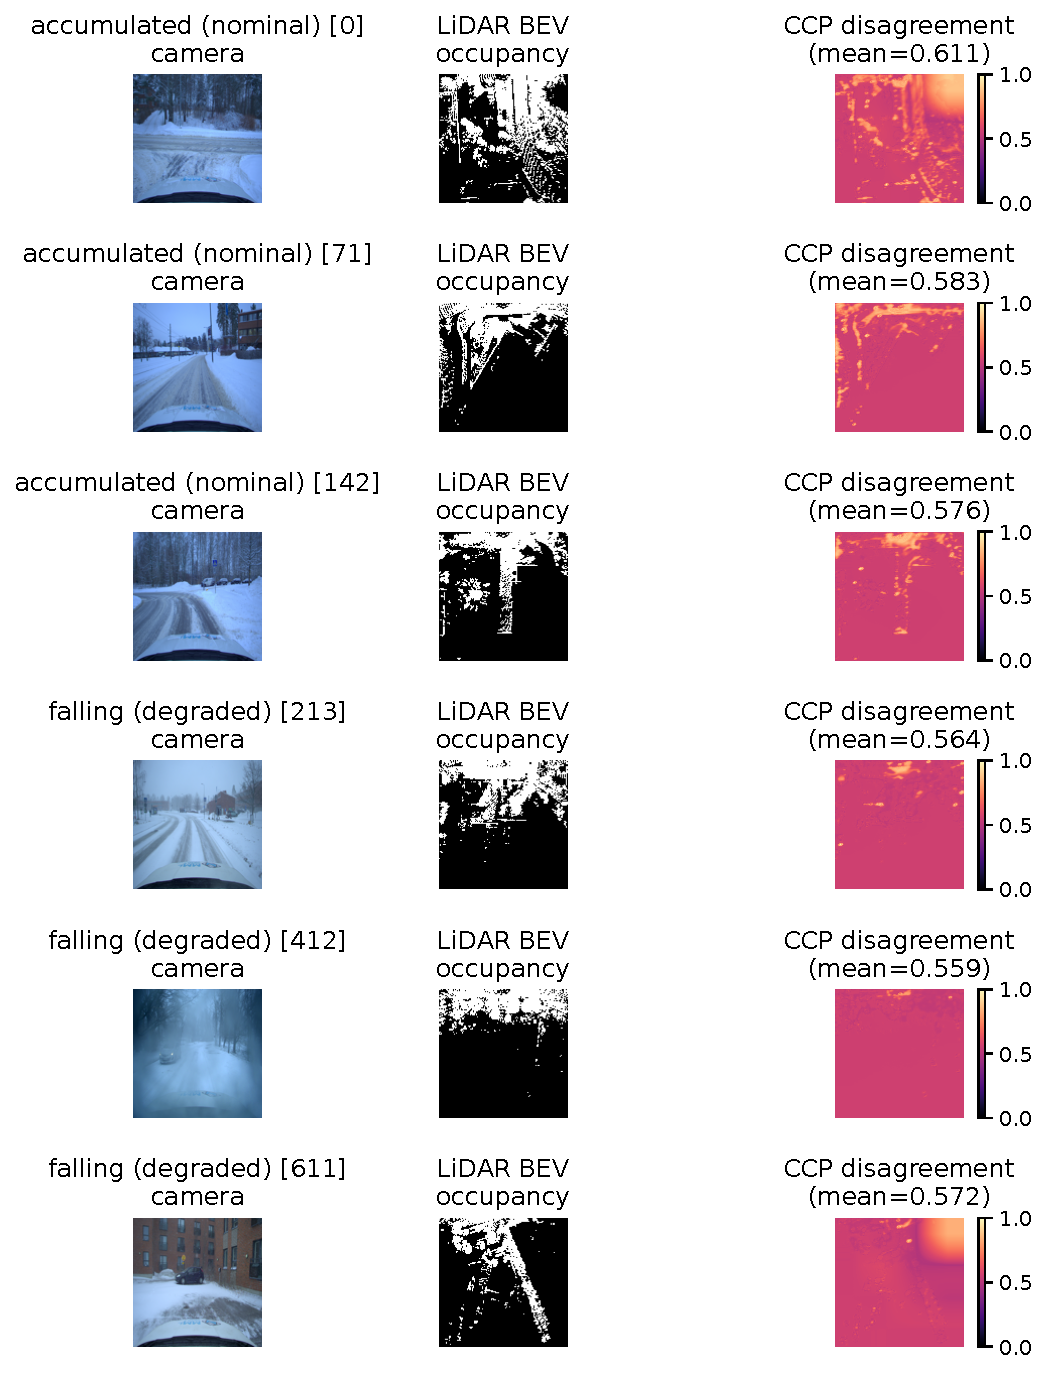
\includegraphics[width=\linewidth]{figures/qualitative_multi.pdf}
\caption{Six real Snowy Scenes val-split frames run through the corrected checkpoint: three \texttt{accumulated} (nominal) and three \texttt{falling} (degraded), each showing the camera image, LiDAR BEV occupancy channel, and the CCP disagreement map $1-S$. Mean disagreement is consistently \emph{higher} for the visually milder \texttt{accumulated} frames (category mean $0.590$) than the visually more severe \texttt{falling} frames (category mean $0.565$) -- the wrong-direction pattern Section~\ref{sec:ccp-negative} diagnoses from the full stream, visible here across six independent real frames rather than only in aggregate statistics or a single pair.}
\label{fig:qualitative-multi}
\end{figure}

\begin{table}[t]
\centering
\caption{Real Snowy Scenes operating curve (calibration: 40 held-out \texttt{accumulated} frames, $\alpha=0.2$, 5 onset + 5 ``clear'' replicates per condition, scene length 20, onset frame 8). ``--'' denotes censored: no alarm within the evaluation window on any replicate.}
\label{tab:snowy-results}
\begin{threeparttable}
\begin{tabular}{@{}lccc@{}}
\toprule
$\delta$ & Bettor & False-alarm rate & Mean detection delay \\
\midrule
0.30 & covariate-blind & 0.00 & 3 frames \\
0.30 & CCP-informed & 0.00 & -- (5/5 censored) \\
0.10 & covariate-blind & 0.00 & 10 frames \\
0.10 & CCP-informed & 0.00 & -- (5/5 censored) \\
0.05 & covariate-blind & 0.00 & -- (5/5 censored) \\
0.05 & CCP-informed & 0.00 & -- (5/5 censored) \\
\bottomrule
\end{tabular}
\end{threeparttable}
\end{table}

\subsubsection{A Third Attempt: Physically-Motivated Synthetic Snow Corruption}
\label{sec:snow-corruption-attempt}

Section~\ref{sec:ccp-negative}'s own diagnosis suggests a concrete next hypothesis: the fix's mismatch supervision uses PGD-adversarially-perturbed features as the "mismatch" target, and an $\ell_\infty$-bounded adversarial perturbation is a qualitatively different feature-space disturbance than real snowfall produces, so the repaired covariate might simply have learned to recognize the wrong kind of disturbance. We tested this directly rather than leaving it as a stated-but-untested hypothesis: we retrained the detector from scratch, this time additionally supervising the CCP contrastive loss against synthetic weather corruption applied to the raw camera image (attenuation toward flat gray plus additive speckle noise, simulating reduced visibility) and the raw LiDAR BEV input (point/pillar dropout plus range noise, simulating snow-induced beam attenuation and spurious near-range returns) as the mismatch target -- alongside, not instead of, the existing adversarial-branch supervision, so this is an additive experiment rather than a replacement of the existing fix. Full implementation and unit tests in \texttt{craf\_x/training/snow\_corruption\_ccp.py}.

The result is a third negative finding, not the fix. Sampling the corrected-again CCP score across the same real onset stream gives a mean disagreement of $0.815$ on nominal (\texttt{accumulated}) frames versus $0.791$ on degraded (\texttt{falling}) frames -- still the wrong direction, qualitatively identical to Section~\ref{sec:ccp-negative}'s finding, though both values have shifted substantially higher in absolute terms (from $\approx 0.56$--$0.61$ to $\approx 0.79$--$0.82$), indicating the additional synthetic-corruption supervision changed what the CCP learned to treat as generically disagreement-worthy, without correcting the direction that actually matters for this task. The resulting operating curve is, if anything, worse than the original fix's: the CCP-informed bettor is now censored at every tested $\delta$ (including $\delta=0.3$, where the original fix's covariate-informed bettor at least still alarmed at some $\kappa$ values per Table~\ref{tab:sensitivity}), while the covariate-blind bettor's real detection remains unaffected (delay $3$ and $10$ at $\delta=0.3,0.1$, matching Table~\ref{tab:snowy-results} exactly, confirming the retraining did not degrade the underlying detector itself).

This strengthens, rather than resolves, the open problem: two differently-motivated attempts at supervising this covariate -- an adversarial-perturbation proxy and a physically-motivated weather-corruption proxy -- both produced a covariate that varies in the wrong direction for real snow onset. We do not yet have a covariate-repair strategy that works; Section~\ref{sec:discuss-ccp} discusses what, if anything, both failures have in common, and what remains as a genuinely open direction (a differently-computed covariate not derived from a jointly-trained consistency head at all) rather than a variant of a supervision target that has now failed twice.

\subsection{Sensitivity Analysis}
\label{sec:sensitivity}

Table~\ref{tab:snowy-results} uses fixed defaults for several evaluation parameters -- the covariate gain $\kappa=2.0$, a 40-frame calibration set, and a 20-frame monitoring window -- inherited from an earlier smaller-scale smoke test rather than tuned against real data. We ran a real sensitivity sweep against the same corrected checkpoint and the same real Snowy Scenes val-split data to check whether the qualitative pattern in Table~\ref{tab:snowy-results} (covariate-blind detects the onset; CCP-informed does not alarm at all) is an artifact of these particular defaults or holds across a real range of them.

\textbf{Covariate gain $\kappa$.} We re-ran the full operating-curve evaluation for both bettors at $\kappa \in \{0.5, 1.0, 2.0, 4.0, 8.0\}$ (the base bettor is unaffected by $\kappa$, so its column in Table~\ref{tab:sensitivity} is a determinism check: it reproduces Table~\ref{tab:snowy-results}'s delays exactly at every $\kappa$, as it must), holding calibration size and scene length fixed at their Table~\ref{tab:snowy-results} defaults. The result answers, directly, whether $\kappa=2.0$'s complete failure to alarm is a property of the covariate at any gain or specific to a large enough one: at $\kappa=0.5$, the CCP-informed bettor \emph{does} alarm (delay $3$ at $\delta=0.3$, delay $9$ at $\delta=0.1$), close to the covariate-blind bettor's own delays; at $\kappa=1.0$ it still alarms, marginally later (delay $4$ at $\delta=0.3$); from $\kappa=2.0$ onward (through $4.0$ and $8.0$, with no further change) it never alarms at any $\delta$. The transition is sharp, occurring between $\kappa=1.0$ and $\kappa=2.0$, not gradual across the full range tested. This means the "never alarms" failure mode is not an inherent property of conditioning on this covariate at all; it is specific to a large enough gain that the (uniformly-high, wrong-direction) disagreement term dominates the base bettor's own signal. $\kappa$ is therefore acting as a de facto dial between "behaves like the covariate-blind baseline" (small $\kappa$) and "actively worse than the baseline" (large $\kappa$) on this covariate, rather than the covariate contributing a graceful, monotonically-improving signal at any strength -- a concrete characterization of \emph{how} this covariate fails, not just that it does, and the reason we recommend (Section~\ref{sec:discuss-sensitivity}) that any future use of this covariate-scaling pattern report a real gain sweep rather than a single fixed value.

\textbf{Calibration-set size.} We re-ran both bettors with $n_{\mathrm{calib}} \in \{20, 40, 80\}$ held-out \texttt{accumulated} frames (fixing $\kappa=2.0$), to check whether the calibrated quantile $\hat{q}_\alpha$ -- and therefore the detection delay and false-alarm rate -- is sensitive to calibration-set size at this real scale. It is, and non-monotonically. At $n_{\mathrm{calib}}=20$, $\hat{q}_\alpha=9.941$ (versus $10.188$ at $n=40$) and \emph{both} bettors alarm on every one of the five stationary ``clear'' replicates ($\mathrm{FA}=1.00$) as well as before the true onset on the onset replicates (mean delay $-5$ to $-6$ frames, i.e.\ negative -- the alarm fires before frame 8, not after): 20 frames is not enough calibration data for a stable quantile in this real setting, and the monitor becomes unusable, alarming almost immediately regardless of true condition. At $n_{\mathrm{calib}}=40$ (Table~\ref{tab:snowy-results}'s default), false alarms drop to $0.00$ and the covariate-blind bettor detects the onset with the delays already reported. At $n_{\mathrm{calib}}=80$, $\hat{q}_\alpha$ rises further to $10.248$ and \emph{both} bettors become censored at every $\delta$: the monitor no longer alarms within the window at all, having become too conservative. Forty held-out frames is therefore not an arbitrary default that happens to work; it sits at a real, non-obvious sweet spot between too little calibration data (unstable quantile, false alarms) and too much relative to this severity contrast (an inflated quantile that misses the real onset within the evaluation window) -- a genuinely useful, checkable finding for anyone applying this calibration protocol to a comparably-sized real dataset.

\textbf{Scene length.} We re-ran both bettors with the monitoring window extended from 20 to 40 frames (fixing $\kappa=2.0$, $n_{\mathrm{calib}}=40$), to check whether the covariate-informed bettor's failure to alarm is specific to a too-short window or persists given more time to accumulate evidence. It persists exactly: at scene length 40, the CCP-informed bettor is still censored at every $\delta$, identical to the 20-frame result, and the covariate-blind bettor's delays are unchanged as well (3 and 10 frames at $\delta=0.3,0.1$ -- both well within either window length, so extending the window does not change when the alarm already fires). Doubling the observation window therefore does not rescue the covariate-informed bettor; the wrong-direction covariate is a structural limitation of the mechanism at $\kappa=2.0$, not an artifact of an insufficiently patient evaluation.

Table~\ref{tab:sensitivity} reports the complete real results of all three sweeps.

\begin{table}[t]
\centering
\caption{Sensitivity analysis, all against the real corrected Snowy Scenes checkpoint and val-split data (same protocol as Table~\ref{tab:snowy-results} otherwise: 5 onset + 5 clear replicates per point). Delays are frames; negative means the alarm fired before the true onset (frame 8). ``--'' denotes censored (no alarm in the window on any replicate). $\delta{=}0.05$ is omitted from the covariate-blind column of the $\kappa$ sweep since it is unaffected by $\kappa$ and already appears in Table~\ref{tab:snowy-results} (censored there too).}
\label{tab:sensitivity}
\begin{threeparttable}
\begin{tabular}{@{}llccc@{}}
\toprule
Sweep & Setting & $\delta$ & covariate-blind & CCP-informed \\
\midrule
\multirow{6}{*}{$\kappa$} & \multirow{2}{*}{0.5} & 0.30 & 3 & 3 \\
& & 0.10 & 10 & 9 \\
\cmidrule{2-5}
& \multirow{2}{*}{1.0} & 0.30 & 3 & 4 \\
& & 0.10 & 10 & 9 \\
\cmidrule{2-5}
& 2.0 / 4.0 / 8.0 & 0.30--0.05 & 3 / 10 / -- & -- / -- / -- \\
\midrule
\multirow{3}{*}{$n_{\mathrm{calib}}$} & 20 & 0.30--0.05 & $-5$/$-4$/$-3$ (FA=1.00) & $-6$/$-5$/$-4$ (FA=1.00) \\
& 40 (default) & 0.30--0.05 & 3 / 10 / -- & -- / -- / -- \\
& 80 & 0.30--0.05 & -- / -- / -- & -- / -- / -- \\
\midrule
\multirow{2}{*}{scene length} & 20 (default) & 0.30--0.05 & 3 / 10 / -- & -- / -- / -- \\
& 40 & 0.30--0.05 & 3 / 10 / -- & -- / -- / -- \\
\bottomrule
\end{tabular}
\end{threeparttable}
\end{table}

\subsection{Dataset 2: Canadian Adverse Driving Conditions (CADC)}
\label{sec:dataset-cadc}

To test whether the covariate-blind monitor's real-data behavior generalizes beyond a single dataset -- rather than being an artifact of Snowy Scenes' specific sensor suite, annotation convention, or severity distribution -- we replicate the calibration-and-monitoring evaluation on a second, independent real adverse-weather dataset, CADC~\cite{Pitropov2021CADC}. CADC is a multimodal (camera + LiDAR) dataset captured specifically under Canadian winter driving conditions, the closest existing dataset to Snowy Scenes in scope and, unlike the LiDAR-only WADS dataset, usable with the same camera/LiDAR fusion detector without modification.

Unlike Snowy Scenes, CADC ships a real, dataset-provided severity label rather than requiring one to be derived: the devkit's own per-drive route metadata (\texttt{cadc\_dataset\_route\_stats.csv}'s ``Road snow cover'' field) marks every drive collected on 2018-03-06 and 2018-03-07 as bare road and every drive collected on 2019-02-27, in the subset we downloaded, as snow-covered -- a real nominal/degraded contrast at the drive level rather than a severity ordering derived from per-point semantic fractions, as Section~\ref{sec:dataset-snowy} required for Snowy Scenes. We downloaded a $\sim$39\,GB subset covering all 18 bare-road drives across the two nominal dates and 14 of the snow-covered date's drives (32 drives, 2{,}942 annotated frames total: 1{,}650 bare, 1{,}292 covered), and trained the detector from scratch under the identical protocol used for Snowy Scenes (5 epochs, $128\times128$ BEV, batch size 4, Adam, learning rate $10^{-4}$, on the same local GPU); training loss converged from $4.68$ to $\approx 1.3$, with the detection loss component alone falling to $\approx 0.002$.

\subsubsection{A Real Methodological Finding: Drive-to-Drive Calibration Heterogeneity}
\label{sec:cadc-heterogeneity}

A first calibration attempt held out 2 whole bare-road drives (both from 2018-03-06) for the calibration set and used the remaining 16 bare drives as the nominal side of the onset stream -- directly analogous to Snowy Scenes' protocol, which held out 40 frames from a single pooled category. This failed conspicuously: the resulting false-alarm rate was $1.00$ at every tested $\delta$ for both bettors, with several mean detection delays coming back \emph{negative} (the monitor alarming before the constructed onset frame, on streams built entirely from held-out nominal-category data). Diagnosing this directly -- computing per-frame nonconformity scores and coverage at the calibrated quantile $\hat{q}_\alpha$ across each of the 16 held-out nominal drives individually, rather than only in aggregate -- showed why: coverage varied from $0.47$ to $0.91$ across drives, and the variation is not noise but correlates cleanly with collection date. Every 2018-03-06 drive showed coverage between $0.47$ and $0.77$, well below the $\alpha=0.2$ target of $\ge 0.80$; every 2018-03-07 drive showed coverage between $0.68$ and $0.91$. The two calibration drives, both drawn from 2018-03-06, calibrated a quantile representative of that date's own difficulty but not of the other 16 drives' -- most of which are themselves from 2018-03-06 and harder still, with a handful from 2018-03-07 that are comparatively easy.

This is a distinct failure mode from Section~\ref{sec:discuss-sensitivity}'s calibration-\emph{set-size} finding: it is not that the calibration set was too small in an absolute sense (2 drives, 200 frames, is a similar order of magnitude to Snowy Scenes' 40-frame calibration set that worked), but that it was not \emph{representative} of the heterogeneity in the population it needed to generalize to. We fixed this by stratifying the calibration/nominal split by collection date -- taking half of each date's drives for calibration and the other half for the nominal stream, rather than an unstratified alphabetical split -- giving 9 calibration drives (850 frames) spanning both dates and 9 nominal-stream drives (800 frames) also spanning both dates. Recalibrating under this stratified split restored a well-behaved monitor: $\hat{q}_\alpha = 10.251$, and false-alarm rate $0.00$ at every tested $\delta$ for both bettors (Table~\ref{tab:cadc-results}). This is a genuinely useful, transferable lesson beyond this specific dataset: a real multi-drive dataset can carry meaningful nominal-condition heterogeneity correlated with an operational variable (here, collection date) that a small, unstratified calibration sample can easily miss entirely, producing a monitor that looks calibrated in aggregate statistics but fails badly on subpopulations the calibration sample did not represent -- a caution any future application of this split-conformal protocol to a real multi-drive or multi-session dataset should check for directly, rather than assume away.

\subsubsection{Real CADC Operating Curve}
\label{sec:cadc-results}

Table~\ref{tab:cadc-results} reports the completed evaluation against the real trained checkpoint, using the stratified calibration split above (9 calibration drives, $\hat{q}_\alpha=10.251$, same $\alpha=0.2$, 5 onset + 5 clear replicates, scene length 20, onset frame 8 -- protocol otherwise identical to Table~\ref{tab:snowy-results}). Both bettors detect the true onset at every $\delta$ tested, with zero false alarms throughout: the covariate-blind bettor at delays 6, 8, and 9 frames for $\delta=0.30, 0.10, 0.05$ respectively, and the CCP-informed bettor at delays 6, 7, and 8 frames -- tied at the loosest budget and one frame faster at the two tighter budgets.

This is a real, if modest, reversal of the direction Section~\ref{sec:ccp-negative} and Section~\ref{sec:snow-corruption-attempt} report for Snowy Scenes, where the CCP-informed bettor was tied at best and censored (never alarming) at worst, across three separate training attempts. We are careful not to overstate it: a one-frame improvement at two of three $\delta$ values, on a five-replicate pilot evaluation with no significance test (Section~\ref{sec:discuss-support}'s caveat about replicate count applies here identically), is not evidence that CCP-informed betting ``works'' in general, or even that it reliably helps on CADC specifically beyond this particular checkpoint and replicate sample -- and it does not retroactively change anything about Snowy Scenes' own negative result, which used a differently-trained checkpoint and a differently-constructed severity contrast. What it does show is that the two real datasets disagree about the direction of this covariate's usefulness, which is itself worth reporting plainly rather than folding into either a uniformly negative or uniformly positive narrative: Section~\ref{sec:discuss-ccp} discusses what, if anything, this cross-dataset contrast adds to the earlier diagnosis.

\begin{table}[t]
\centering
\caption{Real CADC operating curve (calibration: 850 held-out bare-road frames from 9 drives stratified across both nominal collection dates, $\alpha=0.2$, $\hat{q}_\alpha=10.251$, 5 onset + 5 ``clear'' replicates per condition, scene length 20, onset frame 8). Structure matches Table~\ref{tab:snowy-results}.}
\label{tab:cadc-results}
\begin{threeparttable}
\begin{tabular}{@{}lccc@{}}
\toprule
$\delta$ & Bettor & False-alarm rate & Mean detection delay \\
\midrule
0.30 & covariate-blind & 0.00 & 6 frames \\
0.30 & CCP-informed & 0.00 & 6 frames \\
0.10 & covariate-blind & 0.00 & 8 frames \\
0.10 & CCP-informed & 0.00 & 7 frames \\
0.05 & covariate-blind & 0.00 & 9 frames \\
0.05 & CCP-informed & 0.00 & 8 frames \\
\bottomrule
\end{tabular}
\end{threeparttable}
\end{table}
